\documentclass[11pt,a4paper]{article}
\usepackage[top=2cm,bottom=2cm,left=2.5cm,right=2.5cm]{geometry}
\usepackage{xcolor}
\usepackage{tabularx}
\usepackage{array}
\usepackage{colortbl}
\usepackage{listings}
\usepackage{amssymb}
\usepackage{parskip}
\usepackage{graphicx}
\usepackage{fancyhdr}
\usepackage{lastpage}
\usepackage{dashrule}
\usepackage[hidelinks]{hyperref}

% ── Colours ──
\definecolor{navy}{HTML}{1F3864}
\definecolor{grey44}{HTML}{444444}
\definecolor{grey55}{HTML}{555555}
\definecolor{grey77}{HTML}{777777}
\definecolor{greyAA}{HTML}{AAAAAA}
\definecolor{blueBg}{HTML}{F0F4F8}
\definecolor{greenBorder}{HTML}{4A7C3F}
\definecolor{greenBg}{HTML}{F4F8F0}
\definecolor{codeBg}{HTML}{F5F5F5}
\definecolor{codeText}{HTML}{2D2D2D}

% ── Helpers ──
\newcommand{\sectionHead}[1]{\vspace{1.2em}{\Large\bfseries\color{navy}#1}\vspace{0.4em}}

\newcommand{\infobox}[3]{% {title}{text}{border colour}
  \vspace{0.4em}%
  \noindent\fcolorbox{#3}{blueBg}{%
    \begin{minipage}{\dimexpr\textwidth-2\fboxsep-2\fboxrule}%
      {\bfseries\color{#3}#1}\par\smallskip #2%
    \end{minipage}%
  }\vspace{0.4em}%
}

\newcommand{\greenbox}[2]{%
  \vspace{0.4em}%
  \noindent\fcolorbox{greenBorder}{greenBg}{%
    \begin{minipage}{\dimexpr\textwidth-2\fboxsep-2\fboxrule}%
      {\bfseries\color{greenBorder}#1}\par\smallskip #2%
    \end{minipage}%
  }\vspace{0.4em}%
}

\newcommand{\fileref}[2]{%
  \vspace{0.2em}\noindent\texttt{\bfseries #1}~~---~~{\color{grey55}#2}\par
}

\newcommand{\imgplaceholder}[1]{%
  \vspace{0.4em}%
  \noindent\hdashrule{\textwidth}{0.5pt}{2pt 2pt}%
  \begin{center}
    \vspace{1.5cm}
    {\color{greyAA}[IMAGE PLACEHOLDER]}\par\smallskip
    {\small\itshape\color{grey77}#1}
    \vspace{1.5cm}
  \end{center}
  \noindent\hdashrule{\textwidth}{0.5pt}{2pt 2pt}%
  \vspace{0.4em}%
}

% Code listing style
\lstset{
  basicstyle=\small\ttfamily\color{codeText},
  backgroundcolor=\color{codeBg},
  frame=single,
  rulecolor=\color{greyAA},
  framesep=6pt,
  xleftmargin=6pt,
  xrightmargin=6pt,
  breaklines=true,
  showstringspaces=false,
}

\pagestyle{fancy}
\fancyhf{}
\renewcommand{\headrulewidth}{0pt}
\fancyfoot[C]{\small\color{grey77}Task Description \quad---\quad Page \thepage\ of \pageref{LastPage}}

\begin{document}

% ════════════════════════════════════════════════════════════════
% TITLE
% ════════════════════════════════════════════════════════════════
{\LARGE\bfseries\color{navy}Task Description}\par\smallskip
{\color{grey44}Loads Processing for Static Strength Analysis --- Turbine Rear Structure}\par\smallskip
{\small\itshape\color{grey77}This document is intended to be read by the engineer and sets the task scope. Read this document carefully. Take your time and ask questions to the researcher as needed to clarify the scope or details of the task.}\par

% ════════════════════════════════════════════════════════════════
% 1. BACKGROUND
% ════════════════════════════════════════════════════════════════
\sectionHead{1.~Background}

You are a stress engineer working on the static strength analysis of a \textbf{Turbine Rear Structure (TRS)} in an aero engine. The TRS is a structural component after the Low Pressure Turbine that transfers loads among its neighbouring components: LPT Case, Bearing House, Nozzle, Plug and three lugs (port, starboard and failsafe --- active only when the port or starboard lugs fail).

\begin{figure}[h]
  \centering
  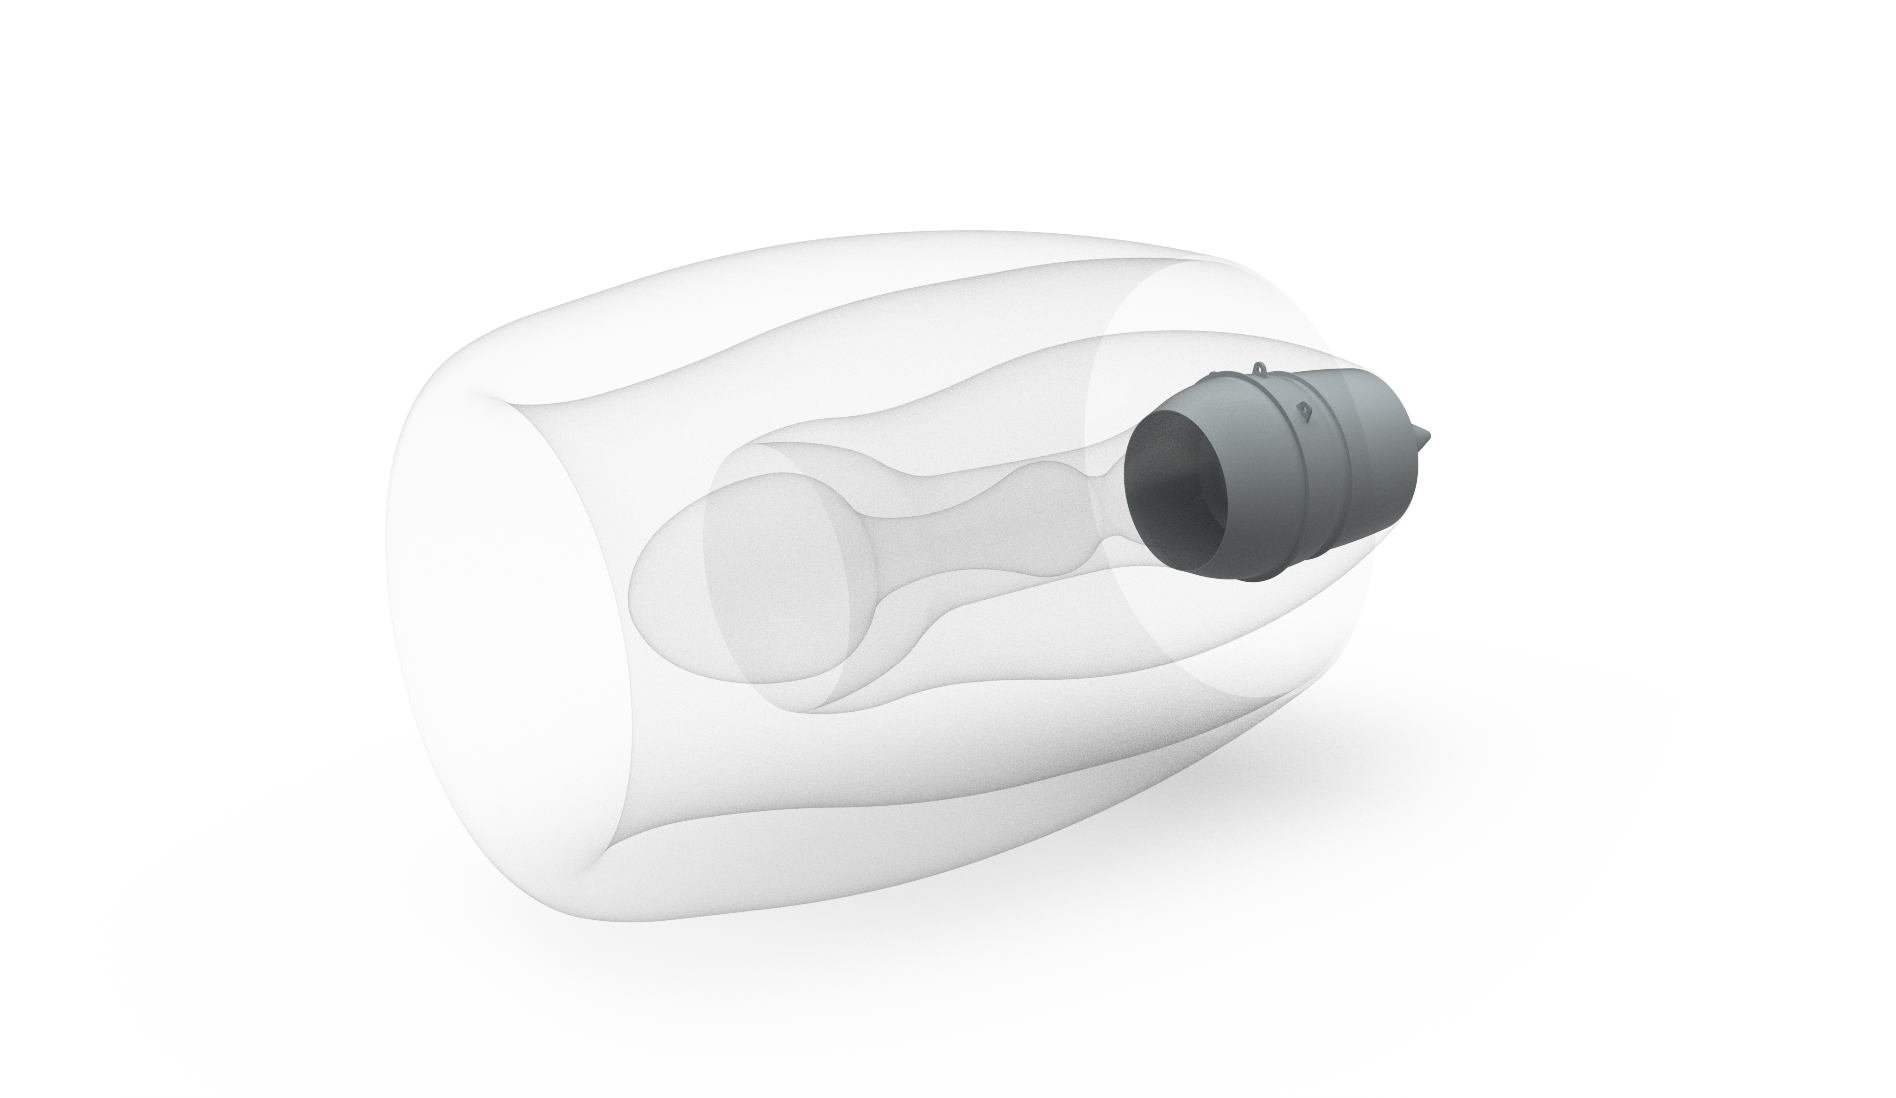
\includegraphics[width=0.70\textwidth]{images/render_1.png}\\[0.5em]
  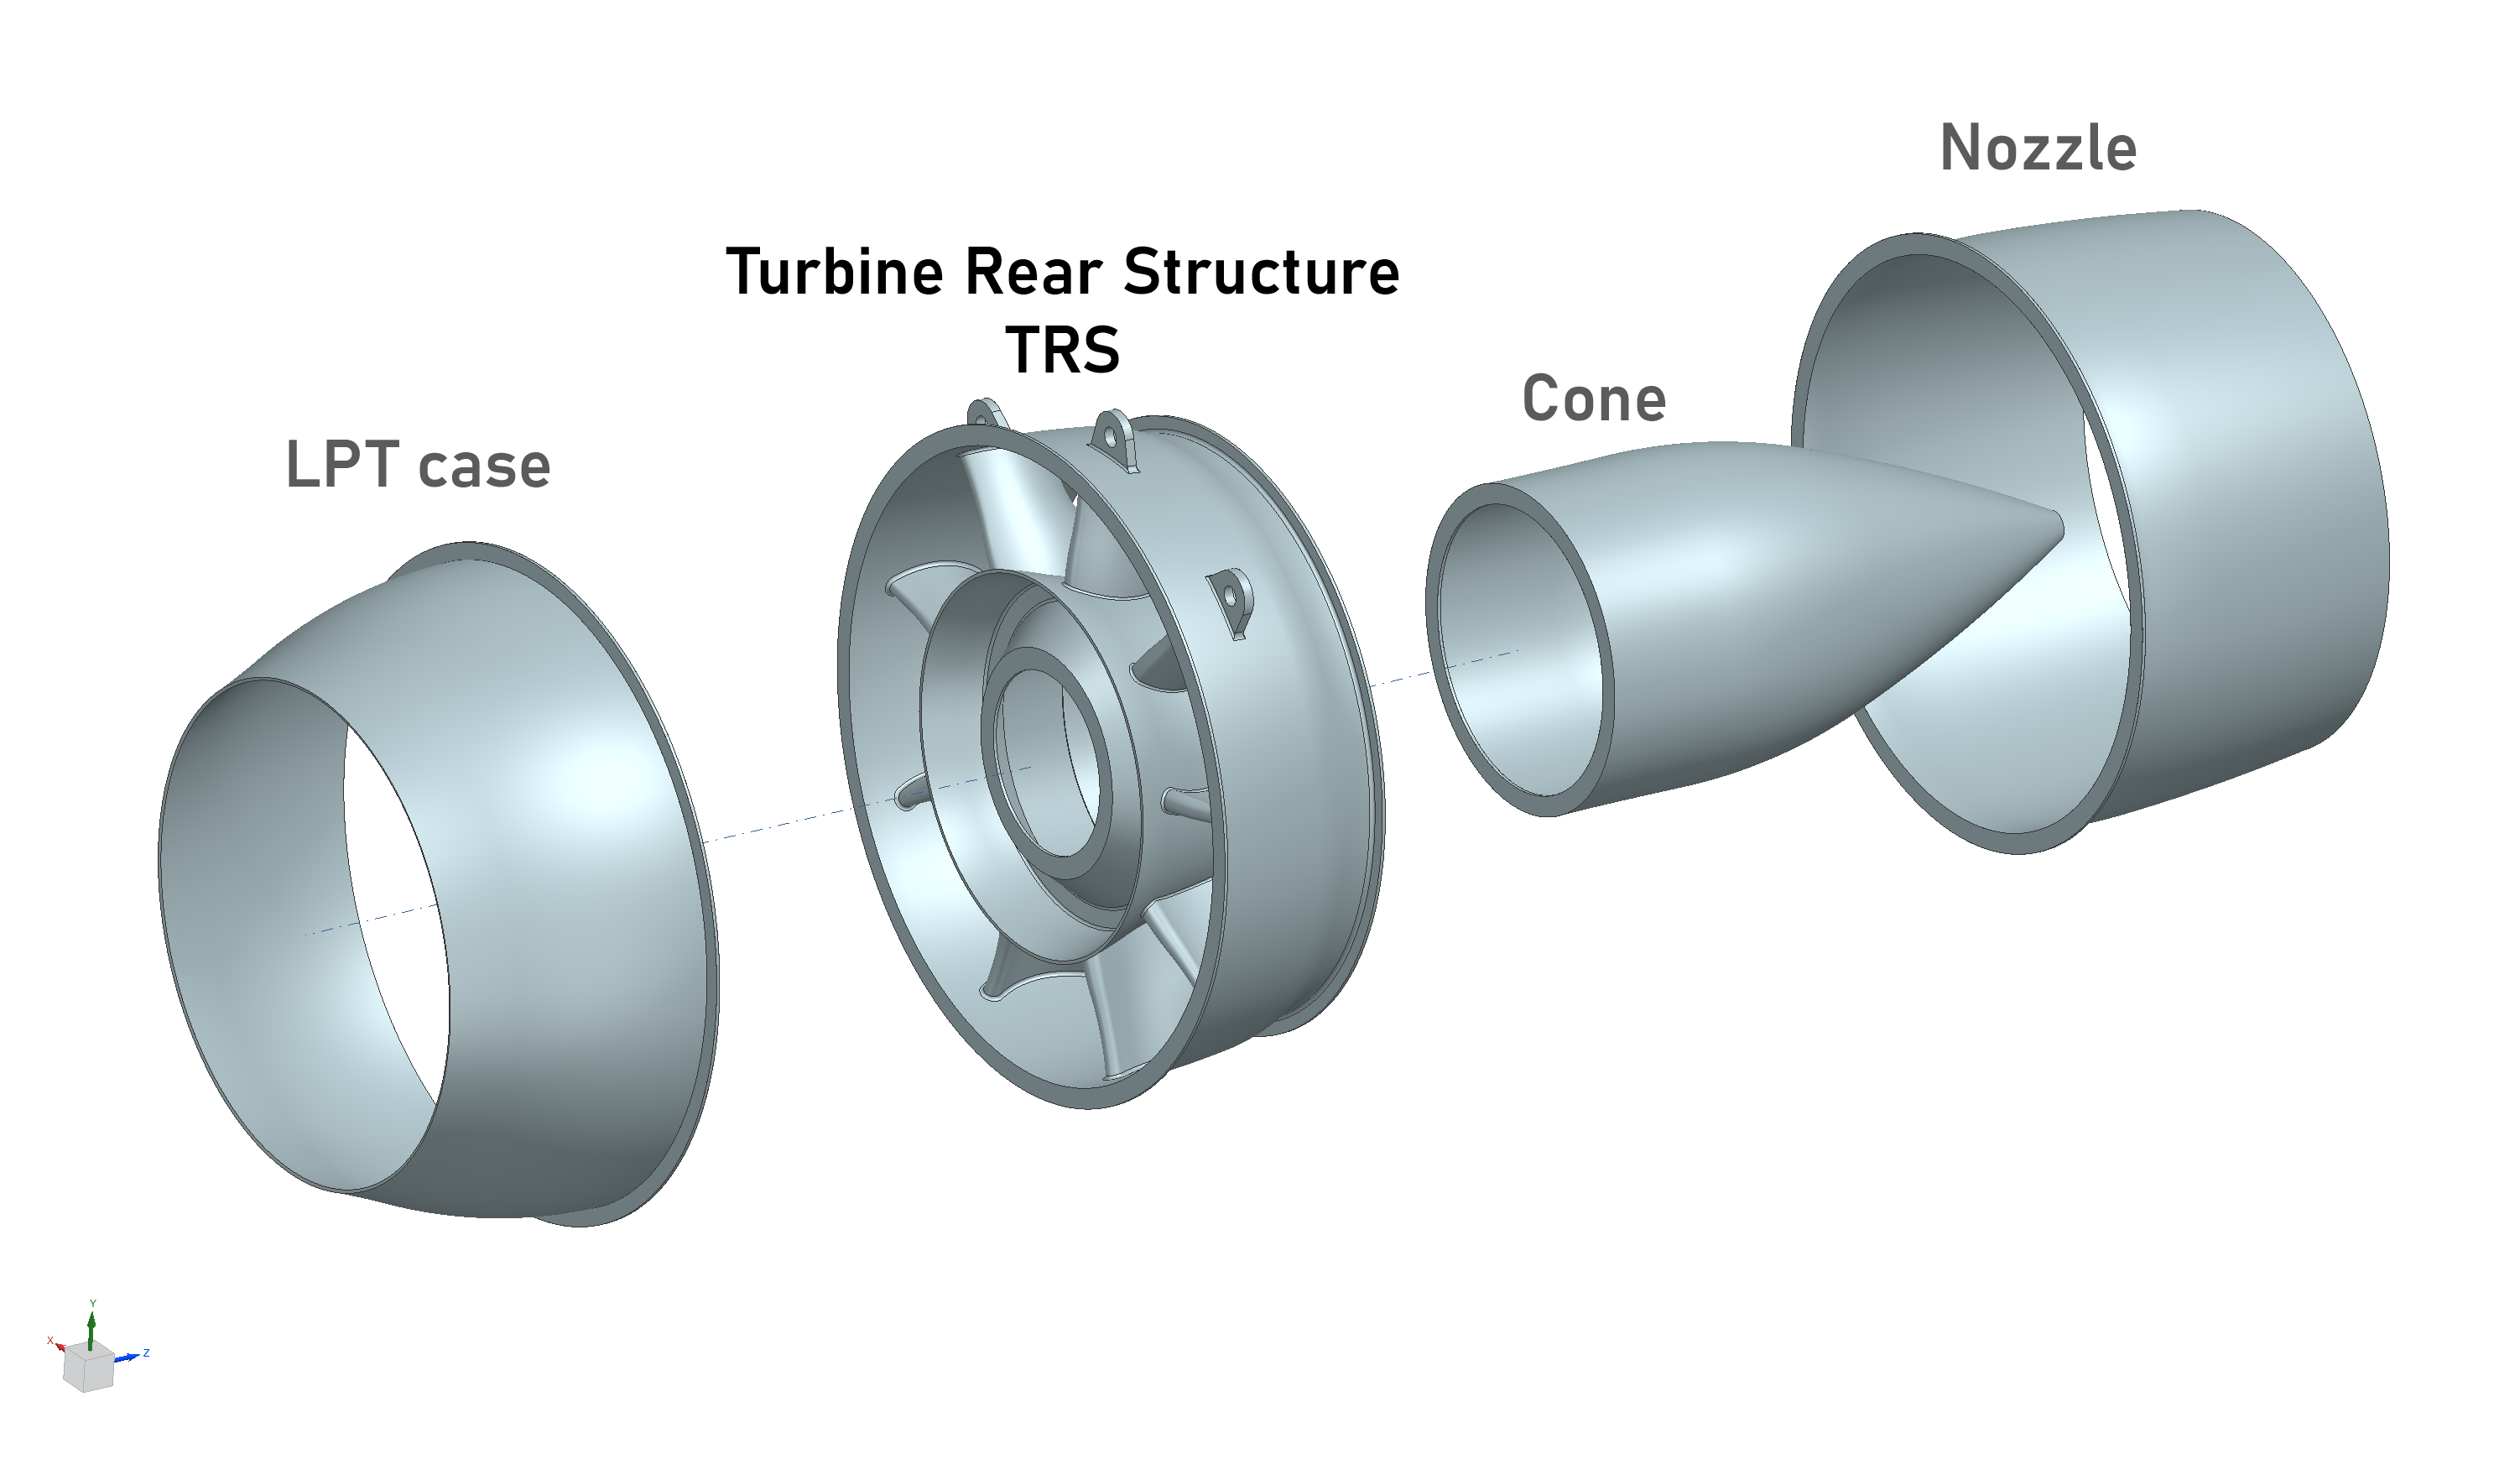
\includegraphics[width=0.70\textwidth]{images/exploded_2_labels_white.png}
  \caption{(top) TRS and neighbouring components positioning on the jet engine and (bottom) neighbouring components in CAD exploded view}
  \label{fig:trs-assembly}
\end{figure}

The programme is in the \textbf{certification phase}. The OEM customer has delivered a new loads update. Your task is to process these loads into input files that can be applied to the Finite Element Model (FEM) for structural analysis. The FE mesh and solver scripts have already been set up by another team member --- running the FE model is not part of this task. The mesh geometry and interface point locations are shown in Figure~\ref{fig:trs-interfaces}. It also shows the equilibrium example of a load case when forces are applied at the interface points.



\begin{figure}[h]
  \centering
  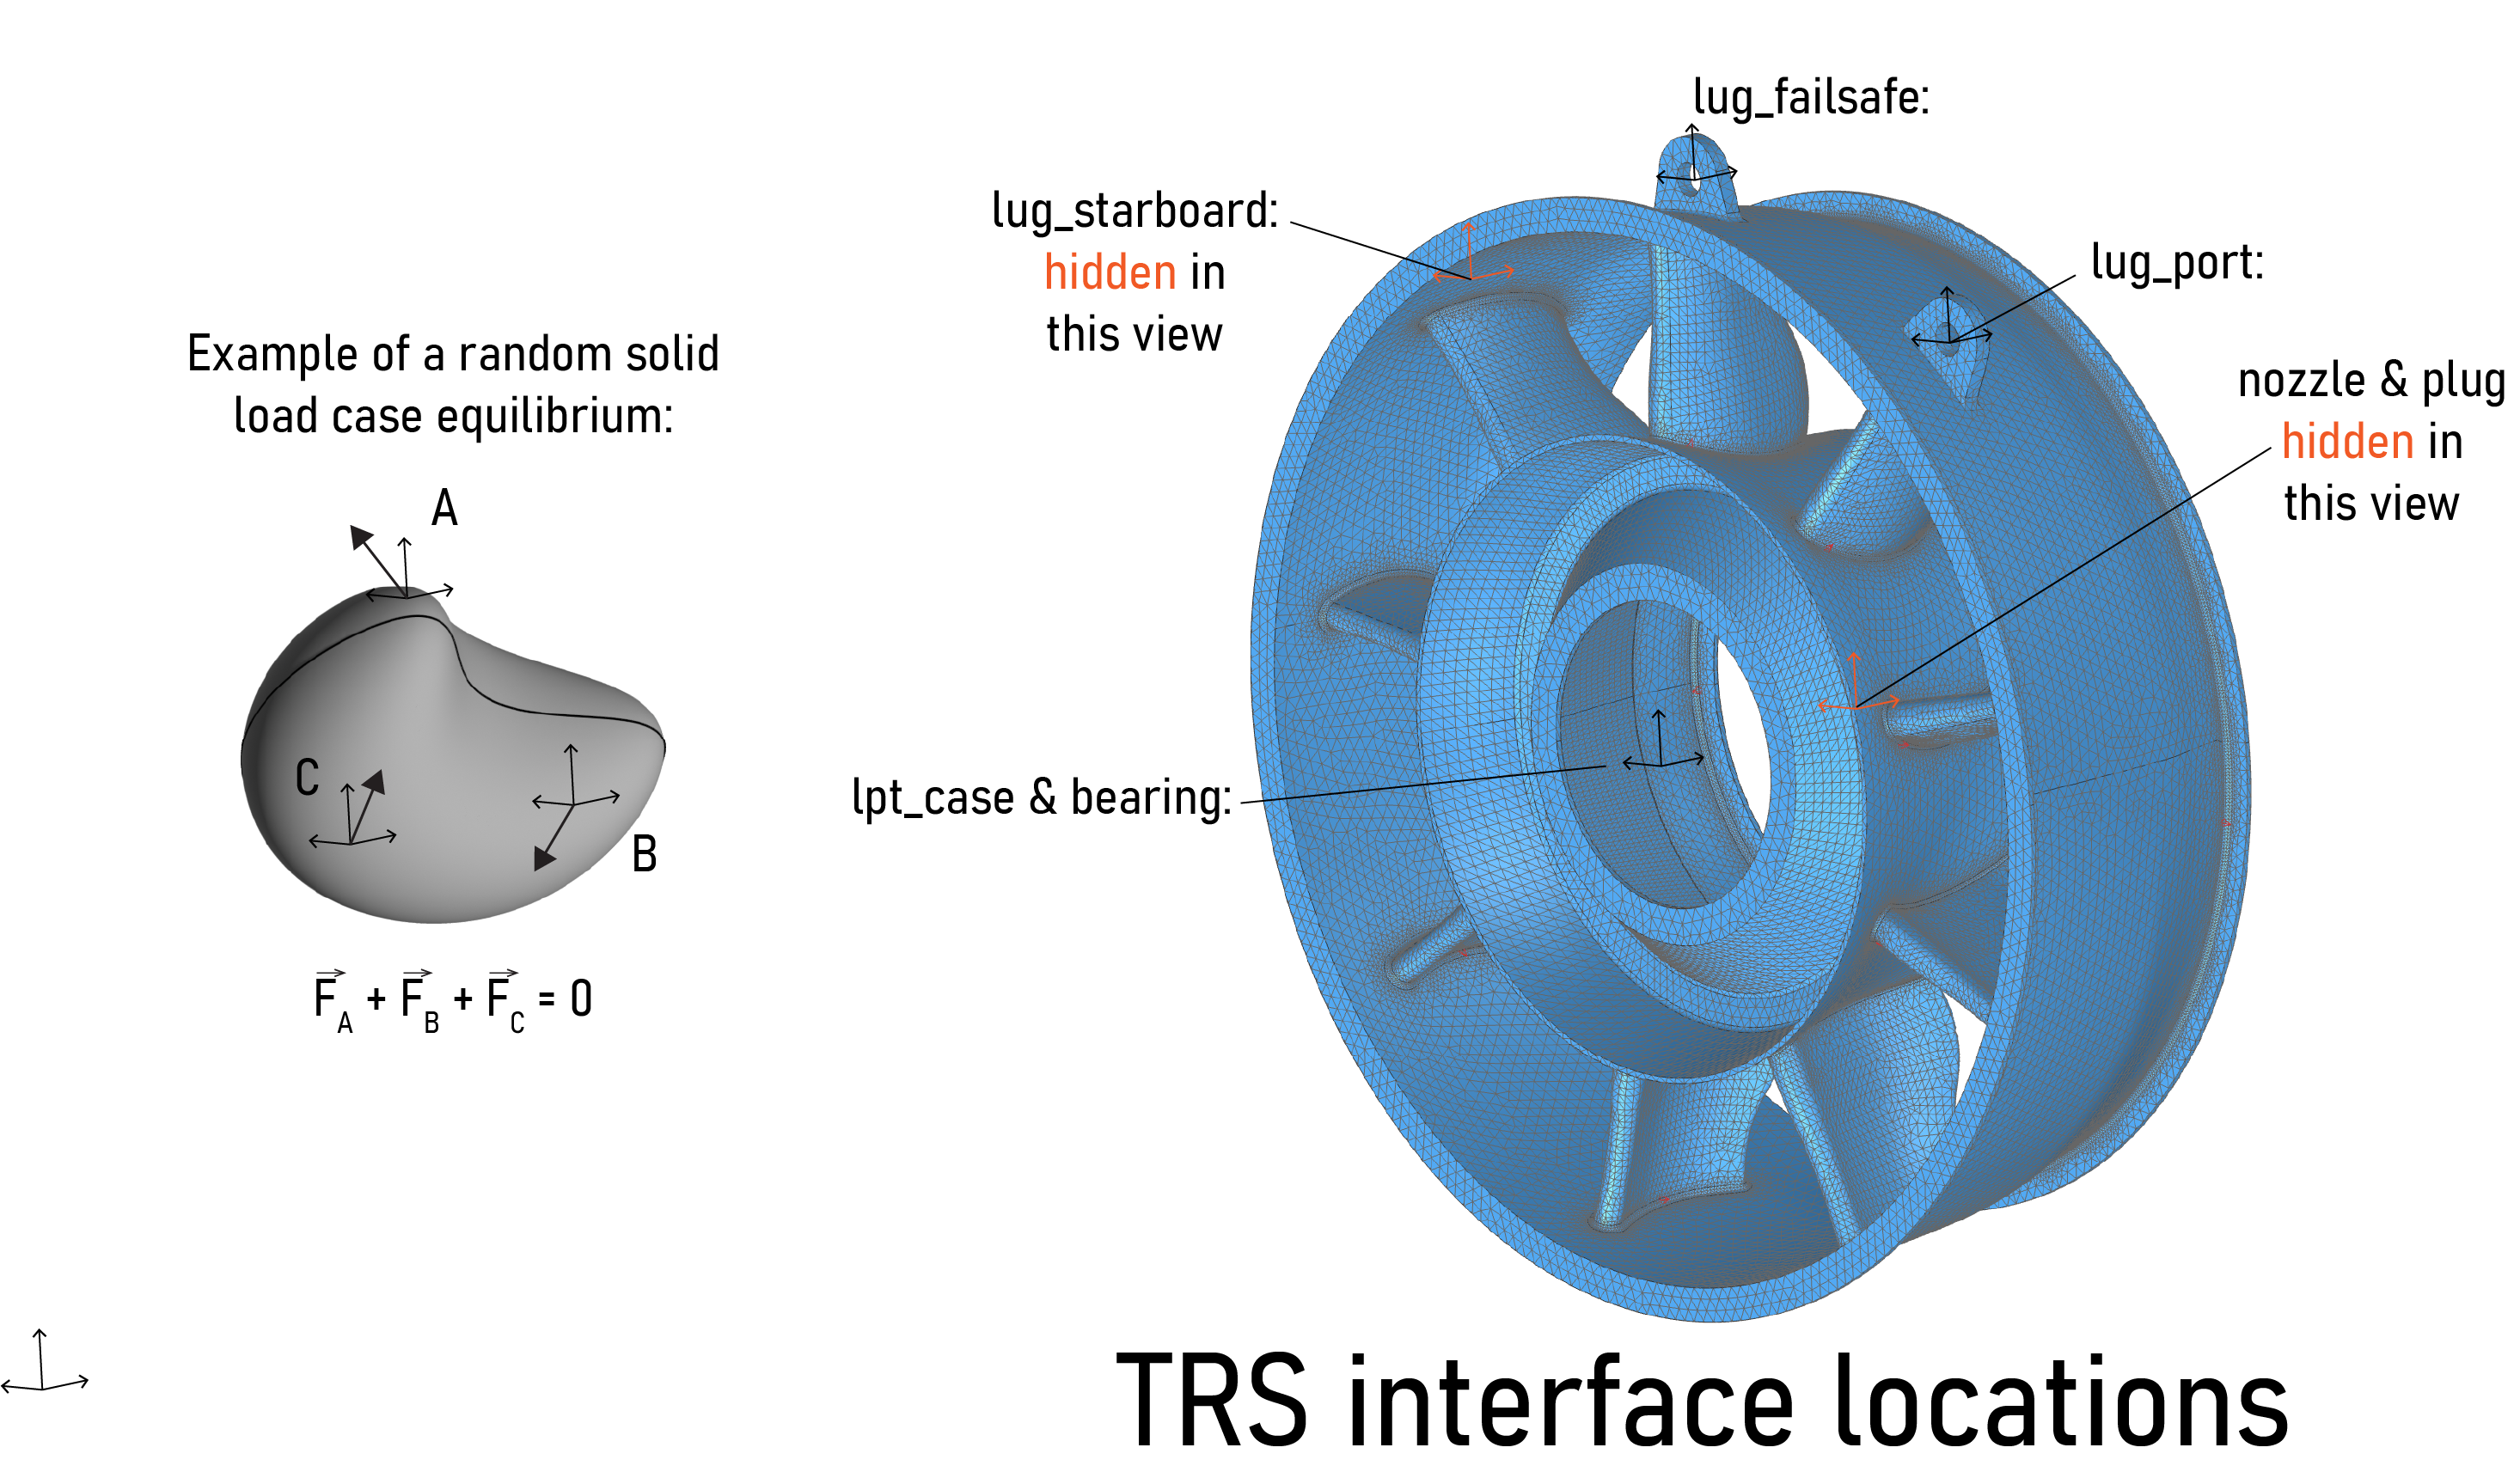
\includegraphics[width=0.85\textwidth]{images/interface locations.png}
  \caption{TRS interface locations showing one loadcase in equilibrium}
  \label{fig:trs-interfaces}
\end{figure}

\newpage
% ════════════════════════════════════════════════════════════════
% 2. YOUR TASK
% ════════════════════════════════════════════════════════════════
\sectionHead{2.~Detailed Task Description}

Your task is to process the new OEM load delivery (\texttt{OEM\_loads\_v2.yaml}) into APDL-ANSYS-compatible input files (\texttt{.inp}), following the methodology document \texttt{loads\_processing\_design\_practice} (document~1001, version~1). The design practice contains all expected processing activities and must be followed in order.

You will use \textbf{Claude Code} (an AI coding agent) to assist you with this task. The agent already has access to the design practice document (document~1001, version~1) --- you do not need to provide it manually.

Make use of the certified tool \texttt{ductile-loads}, available as a Python package on PyPI. Notice that the customer has delivered the files in a different format (YAML) than expected by the tool (JSON). Part of your task is to bypass this limitation.

If there are any loads exceedances, let the researcher know.

\infobox{OEM Correction Notice}{The OEM has informed that due to a human error in the Whole Engine Model export, all \texttt{Fx} force components in this delivery are understated. Apply a \textbf{1.04 multiplication factor to all Fx forces} at every interface point before processing. The OEM has chosen not to issue a revised delivery; the correction shall be applied by the component owner during processing.}{navy}

% ════════════════════════════════════════════════════════════════
% 3. AVAILABLE RESOURCES
% ════════════════════════════════════════════════════════════════
\sectionHead{3.~Available Resources}

The following resources are available:

\begin{itemize}
  \item \textbf{This document} --- a printed copy for you. The agent can also read it from the working directory.
  \item \textbf{Loads processing design practice} --- printed for you. The agent already has access to it. You do not need to give it to the agent.
  \item \textbf{\texttt{ductile-loads}} --- the certified processing tool, available as a Python package on PyPI. The agent can access its documentation online. The documentation is also open in your browser for your reference.
  \item \textbf{Previous analysis} --- script, inputs and outputs in the \texttt{previous\_run/} folder for reference.
\end{itemize}

Additionally, you or the agent can browse the internet and install Python packages via \texttt{uv pip install \textit{package}}.

At any time during the task execution you can ask the researcher for help or clarification, \textit{even half way during the execution of the task}.

% ════════════════════════════════════════════════════════════════
% 4. BEFORE YOU START
% ════════════════════════════════════════════════════════════════
\sectionHead{4.~Before You Start}

\greenbox{Take your time}{This briefing time does not count towards the task duration. Use it to familiarise yourself with the task, the design practice, the tool documentation, and the available files. Check that Claude Code is running in the VS~Code terminal. Feel free to explore the working directory, browse the \texttt{ductile-loads} documentation in your browser, and review the previous analysis. Ask the researcher any questions about the task, the methodology, or the tools --- there are no wrong questions. We will start the timed activity only when you confirm that you are ready.}

\end{document}
